\documentclass{article}

\usepackage[left=2cm,right=2cm,top=2cm,bottom=2cm]{geometry} 

\usepackage[utf8]{inputenc}   % otra alternativa para los caracteres acentuados y la "ñ"
\usepackage[           spanish % para poder usar el español
                      ,es-tabla % para los captions de las tablas
                       ]{babel}   
\decimalpoint %para usar el punto decimal en vez de coma para los números con decimales

%\usepackage{beton}
%\usepackage[T1]{fontenc}

\usepackage{parskip}
\usepackage{xcolor}

\usepackage{caption}

\usepackage{enumerate} % paquete para poder personalizar fácilmente la apariencia de las listas enumerativas

\usepackage{graphicx} % figuras
\usepackage{subfigure} % subfiguras

\usepackage{amsfonts}
\usepackage{amsmath}

\usepackage{listings}
\lstset
{ %Formatting for code in appendix
    language=python,
    basicstyle=\footnotesize,
    stepnumber=1,
    showstringspaces=false,
    tabsize=1,
    breaklines=true,
    breakatwhitespace=false,
}

\definecolor{gris}{RGB}{220,220,220}
	
\usepackage{float} % para controlar la situación de los entornos flotantes

\restylefloat{figure}
\restylefloat{table} 
\setlength{\parindent}{0mm}


\usepackage[bookmarks=true,
            bookmarksnumbered=false, % true means bookmarks in 
                                     % left window are numbered
            bookmarksopen=false,     % true means only level 1
                                     % are displayed.
            colorlinks=true,
            allcolors=blue,
            urlcolor=blue]{hyperref}
\definecolor{webblue}{rgb}{0, 0, 0.5}  % less intense blue


\title{\Huge Inteligencia de Negocio: Práctica 1 \\ Resolución de problemas
  de clasificación y análisis experimental\vspace{10mm}}

\author{\huge David Cabezas Berrido \vspace{10mm} \\ 
  \huge Grupo 2: Viernes \vspace{10mm} \\ \huge dxabezas@correo.ugr.es \vspace{10mm}}

\begin{document}
\maketitle
\newpage
\tableofcontents
\newpage

\section{Introducción}

En esta primera práctica abordaremos el problema de decidir si un
tumor en una mamografía es benigno o maligno, por lo que deducimos que
se trata de un problema de clasificación binaria (dos clases: benigno
y maligno). Disponemos para ello de datos de 961 pacientes, para cada
uno de ellos se han medido 6 atributos entre cualitativos y
cuantitativos.

Sobre este problema real, pondremos a prueba los distintos algoritmos
estudiados en teoría y las herramientas de prácticas. Trataremos de
mejorar los resultados mediante el procesado de los datos y
probando distintos hiperparámetros en los algoritmos. Finalmente,
compararemos los algoritmos entre sí y discutiremos cuál es el más
adecuado para el problema.

Para la experimentación usaremos validación cruzada de 5
particiones. La matriz de confusión se calculará como la suma de las
matrices de confusión de cada partición, de esta forma la matriz
resultante tendrá en cuenta cada instancia una sola vez. Como usamos
validación cruzada, nos ahorramos tener que separar un conjunto de
test para pruebas y aprovechamos cada instancia tanto para
entrenamiento como para evaluación.

Para esta tarea, utilizaremos las herramientas \textit{pandas}, para
tratamiento y visualización de datos; y \textit{sklearn} para el
preprocesado y la creación de los modelos.

Empezamos analizando el dataset. Como ya hemos comentado, consta de
961 instancias y cuenta con 6 atributos: 

\begin{enumerate}
\item Código \href{https://es.wikipedia.org/wiki/BI-RADS}{BI-RADS}: se
  trata de un número entero entre 0 y 6 (ambos incluidos) asignado por
  un radiólogo tras interpretar la mamografía. Un mayor valor
  significa una mayor probabilidad de malignidad, a excepción del
  valor 0, que indica que la información de la radiografía es
  insuficiente. Tendremos que tener esto en cuenta, ya que puede
  ``confundir'' a algunos algoritmos como el KNN, que interpretaría
  que un código 0 está más próximo a un código 1 que a un código 4, lo
  cual no tiene sentido a priori (sin atender a más características).

\item Edad del paciente: entero positivo.
\item Forma del tumor: nominal, 4 posibles formas distintas (R, O, L,
  I) y N para indicar que la forma no está definida.
\item Margen de la masa: nominal, 5 posibles valores (del 1 al 5).
\item Densidad de la masa: entero entre 1 y 4 (ambos inclusive), un
  menor valor indica mayor densidad.
\item Severidad: variable objetivo a predecir, benigno o maligno. 
\end{enumerate}

Hay algunos valores perdidos en el dataset: \vspace{-5mm}
\begin{table}[H]
  \centering
  \begin{tabular}{c|c}
    BI-RADS     & 2 \\
    Age         & 5 \\
    Shape       & 0 \\
    Margin      & 48 \\
    Density     & 76 \\
    Severity    & 0
  \end{tabular}
\end{table}
\vspace{-8mm} En principio, no hay los suficientes valores perdidos como
para dejar de considerar alguna variable, pero durante el procesado de
datos discutiremos si eliminar alguna o cómo imputar los datos
perdidos.

De los 961 instancias, 445 pertenecen a la clase maligno (46.3\%) y
516 a benigno (53.7\%). Las clases están bastante balanceadas, lo que
en general convierte a la accuracy en una métrica bastante adecuada y
fácil de interpretar (proporción de ejemplos bien clasificados) para
la bondad de los algoritmos de clasificación. Sin embargo, en este
problema concreto, parece mucho más grave un falso negativo
(predecimos benigno y enviamos a un paciente a casa que debería
empezar a tratarse) que un falso positivo (predecimos maligno y el
paciente irá a análisis posteriores donde probablemente se percaten
del error); por lo que puede ser interesante considerar otras métricas
de evaluación. También puede ser interesante la métrica
AUC$=\frac{1+\text{TPR}-\text{FPR}}{2}$ (TPR y FPR se definen en la
sección \ref{sec:analisis}), que trata de maximizar el acierto en
ambas clases pero tiene en cuenta si están balanceadas o no (accuracy
no contempla esto).

En concreto, las métricas F1-score y G-measure, medias armónica y
geométrica respectivamente de PPV (proporción de correctas entre las
predicciones positivas) y TPR (proporción de correctas entre los
ejemplos positivos), penalizan más los errores a la hora de clasificar
instancias positias (malignas). Esto las hace más adecuadas para el
problema, por lo que les daremos mayor importancia a la hora de
discutir cuando un algoritmo, configuración o procesamiento es mejor
que otro.

Los algoritmos que pondremosm a prueba son: Árbol de Decisión,
Naive-Bayes, SVM, Random Forest, KNN y Redes Neuronales. Los
introduciremos en la sección \ref{sec:resultados}, excepto los que
configuremos previamente, que los explicaremos en la
\ref{sec:configuracion}.

Todos los procesos aleatorios se realizan con la semilla 185.

\section{Procesado de datos}

Presentamos distintas técnicas de preprocesado de los
datos. Discutiremos, para cada una de ellas, su efecto (bueno o malo)
sobre los resultados de los algoritmos. Para comparar la bondad de los
procesamientos, ejecutaremos todos los algoritmos a comparar con
parámetros por defecto sobre esos datos y atenderemos a los score
medio y máximo conseguidos entre los modelos (ignorando el
\texttt{DummyClassifier}).

En todas ellas debemos usar \texttt{LabelEncoder} (de
\textit{sklearn}), porque los algoritmos de esta librería necesitan
trabajar con datos numéricos.

\subsection{Preprocesado 1: Eliminación de valores perdidos}

La mayoría de los algoritmos no aceptan como entrada datos con valores
perdidos, esto se podría solucionar asignando un valor fijo a estos
valores que represente valor perdido, o simplemente podemos eliminar
los valores perdidos con el método \texttt{dropna} del objeto
\texttt{DataFrame} de \textit{pandas}. Este es un preprocesado muy
básico, prácticamente el justo para que funcionen los algoritmos, y
debería ser superado a medida que experimentemos con procesamientos
más avanzados.

Hay que tener en cuenta que el valor 0 en el código BI-RADS significa
radiografía insuficiente, y el valor N en la forma significa que la
forma no está definida. Así que consideraremos estos valores como
perdidos.

Nos quedamos con 825 instancias, 400 positivias (maligno) y 425
negativas (benigno). Siguen bastante balanceadas.

Ejecutamos los algoritmos sobre estos datos y obtenemos los siguientes
resultados:

\begin{table}[H]
\centering
\caption{Eliminación de instancias con valores perdidos}
\label{tab:dropna}
\begin{tabular}{|lrrrrrrrrrr|}
\hline
 & TP & TN & FP & FN & Acc & TPR & FPR & AUC & F1-score & G-measure\\ \hline
Dummy & 400 & 0 & 425 & 0 & 0.4848 & 1.0 & 1.0 & 0.5 & 0.6531 & 0.6963\\
DecisionTree & 288 & 341 & 84 & 112 & 0.7624 & 0.72 & 0.1976 & 0.7612 & 0.7461 & 0.7466\\
GaussianNB & 341 & 340 & 85 & 59 & 0.8255 & 0.8525 & 0.2 & 0.8263 & 0.8257 & 0.8261\\
SupportVectorM & 331 & 314 & 111 & 69 & 0.7818 & 0.8275 & 0.2612 & 0.7832 & 0.7862 & 0.7872\\
RandomForest & 312 & 345 & 80 & 88 & 0.7964 & 0.78 & 0.1882 & 0.7959 & 0.7879 & 0.7879\\
KNN & 330 & 333 & 92 & 70 & 0.8036 & 0.825 & 0.2165 & 0.8043 & 0.8029 & 0.8032\\
NeuralNetwork & 337 & 332 & 93 & 63 & 0.8109 & 0.8425 & 0.2188 & 0.8118 & 0.812 & 0.8126\\ \hline
Máximo & 341 & 345 & 111 & 112 & 0.8255 & 0.8525 & 0.2612 & 0.8263 & 0.8257 & 0.8261\\
Media & 323.2 & 334.2 & 90.8 & 76.8 & 0.7968 & 0.8079 & 0.2137 & 0.7971 & 0.7935 & 0.7939\\
\hline
\end{tabular}
\end{table}

\subsection{Preprocesado 2: Imputación de valores perdidos}

Rellenamos los valores perdidos con algún valor para no tener que
eliminar una instancia y poder aprovechar así el resto de datos de la
instancia (los no perdidos). Para las variables numéricas,
discutiremos 2 formas de hacer esto: la media y la mediana de la
columna. En cambio las nominales las imputaremos usando la moda.

Para esta tarea utilizamos el objeto SimpleImputer de
\textit{sklearn}, debemos indicarle la estrategia que queremos que
utilice. Como hemos comentado: probaremos \texttt{'mean'} y
\texttt{'median'} para las varaiables numéricas y
\texttt{'most\_frequent'} para las nominales. Antes de continuar, nos
quedaremos con la estrategia para las variables numéricas que consiga
los mejores resultados.

\begin{table}[H]
\centering
\caption{Imputando valores perdidos numéricos con la media}
\label{tab:impute-mean}
\begin{tabular}{|lrrrrrrrrrr|}
\hline
 & TP & TN & FP & FN & Acc & TPR & FPR & AUC & F1-score & G-measure\\ \hline
Dummy & 445 & 0 & 516 & 0 & 0.4631 & 1.0 & 1.0 & 0.5 & 0.633 & 0.6805\\
DecisionTree & 316 & 420 & 96 & 129 & 0.7659 & 0.7101 & 0.186 & 0.762 & 0.7375 & 0.738\\
GaussianNB & 374 & 413 & 103 & 71 & 0.8189 & 0.8404 & 0.1996 & 0.8204 & 0.8113 & 0.8118\\
SupportVectorM & 360 & 393 & 123 & 85 & 0.7836 & 0.809 & 0.2384 & 0.7853 & 0.7759 & 0.7765\\
RandomForest & 338 & 422 & 94 & 107 & 0.7908 & 0.7596 & 0.1822 & 0.7887 & 0.7708 & 0.7709\\
KNN & 341 & 411 & 105 & 104 & 0.7825 & 0.7663 & 0.2035 & 0.7814 & 0.7654 & 0.7654\\
NeuralNetwork & 365 & 410 & 106 & 80 & 0.8065 & 0.8202 & 0.2054 & 0.8074 & 0.7969 & 0.7973\\ \hline
Máximo & 374 & 422 & 123 & 129 & 0.8189 & 0.8404 & 0.2384 & 0.8204 & 0.8113 & 0.8118\\
Media & 349 & 411.5 & 104.5 & 96 & 0.7914 & 0.7843 & 0.2025 & 0.7909 & 0.7763 & 0.7766\\
\hline
\end{tabular}
\end{table}

\begin{table}[H]
\centering
\caption{Imputando valores perdidos numéricos con la mediana}
\label{tab:impute-median}
\begin{tabular}{|lrrrrrrrrrr|}
\hline
 & TP & TN & FP & FN & Acc & TPR & FPR & AUC & F1-score & G-measure\\ \hline
Dummy & 445 & 0 & 516 & 0 & 0.4631 & 1.0 & 1.0 & 0.5 & 0.633 & 0.6805\\
DecisionTree & 318 & 420 & 96 & 127 & 0.768 & 0.7146 & 0.186 & 0.7643 & 0.7404 & 0.7409\\
GaussianNB & 374 & 413 & 103 & 71 & 0.8189 & 0.8404 & 0.1996 & 0.8204 & 0.8113 & 0.8118\\
SupportVectorM & 360 & 393 & 123 & 85 & 0.7836 & 0.809 & 0.2384 & 0.7853 & 0.7759 & 0.7765\\
RandomForest & 335 & 420 & 96 & 110 & 0.7856 & 0.7528 & 0.186 & 0.7834 & 0.7648 & 0.7649\\
KNN & 346 & 414 & 102 & 99 & 0.7908 & 0.7775 & 0.1977 & 0.7899 & 0.7749 & 0.7749\\
NeuralNetwork & 366 & 410 & 106 & 79 & 0.8075 & 0.8225 & 0.2054 & 0.8085 & 0.7983 & 0.7986\\ \hline
Máximo & 374 & 420 & 123 & 127 & 0.8189 & 0.8404 & 0.2384 & 0.8204 & 0.8113 & 0.8118\\
Media & 349.8 & 411.7 & 104.3 & 95.2 & 0.7924 & 0.7861 & 0.2022 & 0.792 & 0.7776 & 0.7779\\
\hline
\end{tabular}
\end{table}

Atendiendo al máximo y a la media de los scores de los algoritmos,
observamos que con este preprocesado decrecen levemente las métricas
Accuracy y AUC (Area Under Curve), que miden la eficiencia general de
los modelos. Lo misimo le ocurre a las métricas F1-score y G-measure,
que son las que se ajustan más a la naturaleza del problema, ya que
penalizan más los falsos negativos. Esto ocurre para las dos
estrategias. Aunque la imputación de valores numéricos por la mediana
ha resultado ligeramente mejor que usando la media (es por ellos que
en las secciones \ref{sec:resultados} y \ref{sec:analisis}
consideraremos únicamente la imputación de datos numéricos con la
mediana), ambas han empeorado el desempeño de los algoritmos. Por esto
decidimos abandonar la idea de imputar valores y mantenemos las
instancias con valores perdidos eliminadas. Nos quedamos por tanto con
datos de 825 pacientes.

\subsection{Preprocesado 3: Eliminación de características innecesarias}

Estudiaremos si todas las características son útiles a la hora de
predecir. En primer lugar, obtenemos la desviación típica de cada una:

\begin{table}[H]
  \centering
  \begin{tabular}{cccc}
    BI-RADS &  Age & Margin & Density \\ \hline
	0.635706 & 14.480131 & 1.566546 & 0.380444
  \end{tabular}
\end{table}
Observamos una baja varianza en BI-RADS y en Density, usamos
\texttt{Counter} para ver su distribución y observamos que de las 825
instancias sin valores perdidos, hay 468 con el valor 4 para el código
BI-RADS y 317 con el valor 5. Decidimos mantenerla, ya que puede
seguir teniendo interés, aun así, optamos por colapsar el resto de
valores en 4 (los valores 2 y 3) y 5 (valor 6), ya que hay muy pocas
instancias con estos valores (40 en total). 

En el caso de Density, 750 instancias tienen el valor 3, por lo que su
distribución es prácticamente degenerada en 3. Así que decidimos
eliminar esta variable.

Estas dos acciones suponen obviamente una pérdida de información, pero
ayuda a reducir la complejidad de los modelos y los hace más
fácilmente interpretables, de modo que mantendremos esta decisión
siempre que no suponga un descenso notable en el desempeño de los
algoritmos.

No nos muestra la desviación de Shape al no ser numérica, pero
obtenemos igualmente su distribución con \texttt{Counter} y observamos
que está lejos de ser degenerada, así que la mantenemos.

Con el método \texttt{corr} de \texttt{pandas.DataFrame}, obtenemos la
matriz de correlación entre las características. Si encontrásemos dos
atributos altamente correlados, nos plantearíamos si quedarnos con
sólo uno de ellos.

\begin{figure}[H]
  \centering
  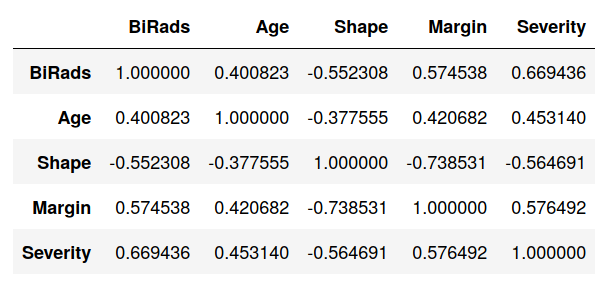
\includegraphics[width=100mm]{figures/corr}
  \caption{Matriz de correlación entre los atributos}
  \label{fig:corr}
\end{figure}

No encontramos ningun par de variables con una correlación alta entre
ellas, el máximo es -0.7385 entre Shape y Margin. De modo que
mantenemos el resto de características.

Los resultados obtenidos son:

\begin{table}[H]
\centering
\caption{Simplificando el conjunto de atributos}
\label{tab:features}
\begin{tabular}{|lrrrrrrrrrr|}
\hline
 & TP & TN & FP & FN & Acc & TPR & FPR & AUC & F1-score & G-measure\\ \hline
Dummy & 400 & 0 & 425 & 0 & 0.4848 & 1.0 & 1.0 & 0.5 & 0.6531 & 0.6963\\
DecisionTree & 293 & 349 & 76 & 107 & 0.7782 & 0.7325 & 0.1788 & 0.7768 & 0.762 & 0.7626\\
GaussianNB & 346 & 347 & 78 & 54 & 0.84 & 0.865 & 0.1835 & 0.8407 & 0.8398 & 0.8402\\
SupportVectorM & 330 & 310 & 115 & 70 & 0.7758 & 0.825 & 0.2706 & 0.7772 & 0.7811 & 0.7822\\
RandomForest & 313 & 345 & 80 & 87 & 0.7976 & 0.7825 & 0.1882 & 0.7971 & 0.7894 & 0.7894\\
KNN & 328 & 335 & 90 & 72 & 0.8036 & 0.82 & 0.2118 & 0.8041 & 0.802 & 0.8022\\
NeuralNetwork & 323 & 338 & 87 & 77 & 0.8012 & 0.8075 & 0.2047 & 0.8014 & 0.7975 & 0.7976\\ \hline
Máximo & 346 & 349 & 115 & 107 & 0.84 & 0.865 & 0.2706 & 0.8407 & 0.8398 & 0.8402\\
Media & 322.2 & 337.3 & 87.7 & 77.8 & 0.7994 & 0.8054 & 0.2063 & 0.7996 & 0.7953 & 0.7957\\
\hline
\end{tabular}
\end{table}

Al comparar los resultados de los algoritmos sobre este procesamiento
con los mejores resultados obtenidos hasta el momento (eliminación de
valores perdidos, Tabla \ref{tab:dropna}), apreciamos una leve mejora
en las métricas Accuracy y AUC, por lo que no ha decaído su capacidad
de predicción. También mejoran levemente los scores F1-score y
G-measure, por lo que los modelos siguen siendo apropiados para el
problema. Esto se debe sobre todo al aumento del desempeño de Gaussian
Naive-Bayes, que supone que los atributos son independientes. Al
simplificar el conjunto de atributos es lógico que disminuya el grado
de dependencia entre los mismos y el algoritmo funcione mejor.

No sólo no hemos observado un descenso en el desempeño de los modelos,
sino una pequeña mejora. Así que mantenemos este preprocesamiento.

\subsection{Preprocesado 4: Binarización de características nominales}

Nuestro dataset tiene dos características nominales: Shape y Margin,
que toman 4 y 5 posibles valores respectivamente. Codificar estas
variables utilizando números naturales puede confundir a algunos
algoritmos. Este es el caso de KNN, que podría interpretar que una
instancia con valor 2 en cualquiera de estas características está más
cerca de una con valor 1 ó 3 que de una con valor 4, cuando no es
lógico pensar esto, ya que estos números simplemente codifican
cualidades. Es por ello que binarizamos estas dos variables
introduciendo 9 nuevos atributos binarios (valdrán 0 ó 1), 4 de ellos
indicarán el valor de Shape (1 en la posición correspondiente al valor
y 0 en las demás) y 5 para el valor de Margin. De esa forma, dos
individuos con distintos valores de la característica Shape estarán a
distancia 0 (por lo que a la variable Shape respecta) si tienen el
mismo valor en esta característica y a una distancia constante
positiva (por lo que a la variable Shape respecta) si tienen valor de
Shape diferente; y análogo para Margin. Esto puede mejorar la
eficiencia de algunos algoritmos, especialmente de KNN.

En este caso, el número de características nominales y de valores que
pueden tomar es bajo, así que esta operación es factible. De haber
existido un número más elevado de características nominales o un
número más elevado de posibles valores para las mismas, binarizar
estas características conllevaría un aumento notable del número de
variables, lo que puede provocar dificultades en el aprendizaje de los
modelos si el número de datos no es lo suficientemente grande.

Para esta tarea utilizamos \texttt{OneHotEnconder}, de
\textit{sklearn}. Los resultados obtenidos son:

\begin{table}[H]
\centering
\caption{Binarización de atributos nominales}
\label{tab:binarization}
\begin{tabular}{|lrrrrrrrrrr|}
\hline
 & TP & TN & FP & FN & Acc & TPR & FPR & AUC & F1-score & G-measure\\ \hline
Dummy & 400 & 0 & 425 & 0 & 0.4848 & 1.0 & 1.0 & 0.5 & 0.6531 & 0.6963\\
DecisionTree & 297 & 347 & 78 & 103 & 0.7806 & 0.7425 & 0.1835 & 0.7795 & 0.7665 & 0.7669\\
GaussianNB & 354 & 321 & 104 & 46 & 0.8182 & 0.885 & 0.2447 & 0.8201 & 0.8252 & 0.8271\\
SupportVectorM & 281 & 307 & 118 & 119 & 0.7127 & 0.7025 & 0.2776 & 0.7124 & 0.7034 & 0.7034\\
RandomForest & 319 & 344 & 81 & 81 & 0.8036 & 0.7975 & 0.1906 & 0.8035 & 0.7975 & 0.7975\\
KNN & 332 & 332 & 93 & 68 & 0.8048 & 0.83 & 0.2188 & 0.8056 & 0.8048 & 0.8052\\
NeuralNetwork & 342 & 337 & 88 & 58 & 0.823 & 0.855 & 0.2071 & 0.824 & 0.8241 & 0.8246\\ \hline
Máximo & 354 & 347 & 118 & 119 & 0.823 & 0.885 & 0.2776 & 0.824 & 0.8252 & 0.8271\\
Media & 320.8 & 331.3 & 93.7 & 79.2 & 0.7905 & 0.8021 & 0.2204 & 0.7908 & 0.7869 & 0.7874\\
\hline
\end{tabular}
\end{table}

Comparamos los resultados con los de la Tabla \ref{tab:features}. Las
métricas Acc. y AUC (que miden la eficacia general de los modelos) han
mejorado levemente en la mayoría de modelos, aunque ha decaído el
máximo score, ya que el mejor modelo hasta el momento (Gaussian
Naive-Bayes) ha visto empeorados sus resultados, la media ha decrecido
porque los resultados de SVM han empeorado drásticamente. No
experimentamos una mejora sustancial en KNN como esperábamos, pero sí
en la Red Neuronal, que también puede sufrir de la condición que hemos
comentado antes, y se convierte en el nuevo máximo. Respecto a las
métricas F1-score y G-measure, que reflejan mejor la naturaleza del
problema, ha ocurrido exactamente lo mismo con la excepción de que la
caída de Gaussian Naive-Bayes y el crecimiento de la Red Neuronal no
han sido suficientes para que la red supere a Naive-Bayes en estas
métricas. Esto ocurre porque la Red Neuronal ha mejorado a Naive-Bayes
gracias a una mejor clasificación en las instancias negativas, a las
que las métricas F1-score y G-measure les dan una menor importancia.

Aquí se nos plantea una elección difícil sobre cual sería mejor
procesamiento, podemos mantener el que teníamos y apostar por
Naive-Bayes; o adoptar el nuevo, y disponer de una gama más amplia
pero hasta ahora menos efectiva de algoritmos. Nos decantaremos por
binarizar los atributos nominales, debido al poco interés que se le ha
dado a Naive-Bayes en clase de teoría y la facilidad de interpretación
que poseen los árboles.

\subsection{Preprocesado 5: Reescalado de los datos}

Otro problema de los datos que puede provocar dificultades en el
aprendizaje de los algoritmos es el hecho de que los datos tengan
distinta naturaleza y por tanto distinta escala. Pongaos un ejemplo:
si una variable toma valores de un orden entre 10 y 100 como es la
edad, y otra variable toma valores entre 20000 y 200000 como podrían
ser ingresos anuales en euros. Un algoritmo como KNN o Red Neuronal,
interpretaría que 20 años de diferencia entre dos sujetos equivaldría
a 20 euros al año de diferencia en sus ingresos, lo cual no es lógico
pensar. Es por esto que algunas variables estarían teniendo un papel
más relevante que otras, según su naturaleza. En nuestro caso, la
variable Age estaría cobrando más relevancia que otras.

Para solucionar este problema recurrimos a un reescalado de las
variables, de tal forma que todas tengan media 0 y desviación típica
1. Utilizamos para ello el objeto \texttt{StandardScaler} de
\textit{sklearn}.

\begin{table}[H]
\centering
\caption{Estandarizando los datos}
\label{tab:stdScaler}
\begin{tabular}{|lrrrrrrrrrr|}
\hline
 & TP & TN & FP & FN & Acc & TPR & FPR & AUC & F1-score & G-measure\\ \hline
Dummy & 400 & 0 & 425 & 0 & 0.4848 & 1.0 & 1.0 & 0.5 & 0.6531 & 0.6963\\
DecisionTree & 297 & 347 & 78 & 103 & 0.7806 & 0.7425 & 0.1835 & 0.7795 & 0.7665 & 0.7669\\
GaussianNB & 354 & 321 & 104 & 46 & 0.8182 & 0.885 & 0.2447 & 0.8201 & 0.8252 & 0.8271\\
SupportVectorM & 333 & 364 & 61 & 67 & 0.8448 & 0.8325 & 0.1435 & 0.8445 & 0.8388 & 0.8388\\
RandomForest & 320 & 341 & 84 & 80 & 0.8012 & 0.8 & 0.1976 & 0.8012 & 0.796 & 0.796\\
KNN & 324 & 350 & 75 & 76 & 0.817 & 0.81 & 0.1765 & 0.8168 & 0.811 & 0.811\\
NeuralNetwork & 333 & 355 & 70 & 67 & 0.8339 & 0.8325 & 0.1647 & 0.8339 & 0.8294 & 0.8294\\ \hline
Máximo & 354 & 364 & 104 & 103 & 0.8448 & 0.885 & 0.2447 & 0.8445 & 0.8388 & 0.8388\\
Media & 326.8 & 346.3 & 78.7 & 73.2 & 0.816 & 0.8171 & 0.1851 & 0.816 & 0.8111 & 0.8115\\
\hline
\end{tabular}
\end{table}

Comparando con la Tabla \ref{tab:binarization}, en las métricas Acc.,
AUC, F1-score y G-measure apreciamos una gran mejora en todos los
algoritmos salvo los árboles y en Naive-Bayes que acostumbran a tratar
las características individualmente (los árboles en cada nodo trabajan
con una única característica). La mayor mejora se observa en SVM, este
algoritmo se beneficia bastante de la estandarización, y esto nos hace
pensar que su mal desempeño anterior ocurrió porque al binarizar las
características nominales reducimos aun más su escala. Pasamos de
características con valores del 1 al 4 (Shape) ó 5 (Margin), a un
número más elevado de características binarias. Esto supone que exista
más diferencia de escalas con respecto a Age, lo que claramente
observamos que perjudica a SVM.

Tras este análisis comparativo de los preprocesados, llegamos a este
último, que combina las diferentes decisiones que hemos ido tomando
(cada técnica de preprocesamiento se ha aplicado sobre la mejor de las
anteriores). Éste será el procesamiento sobre el que configuremos los
modelos.

\section{Configuración de algoritmos} \label{sec:configuracion}

Ajustaremos los hiperparámetros de algunos algoritmos con el fin de
mejorar su desempeño, probaremos los modelos con distinos
hiperparámetros sobre los datos del preprocesado 5, que es el que
hemos elegido como el más adecuado. La excepción está en modelos que
no se vean afectados por el reescalado, como es el caso de los
árboles, para los que utilizaremos el preprocesado 4.

Configuraremos los modelos: Árbol de decisión, Support Vector Machine,
Random Forest, KNN y Neural Network.

No configuraremos el modelo Dummy por razones obvias, ni Naive-Bayes
por la poca importancia que se le ha prestado en clase de teoría.

\subsection{Árbol de Decisión}

Los árboles de decisión son modelos eficaces y fáciles de
interpretar. Partiendo de todos los ejemplos de entrenamiento,
seleccionan en cada nodo atributos para dividir el conjunto de
ejemplos de forma que los subconjuntos generados sean lo más ``puros''
(predomine una clase) posible. Para esto utilizaremos el índice de
impureza
\href{https://es.wikipedia.org/wiki/Aprendizaje_basado_en_%C3%A1rboles_de_decisi%C3%B3n#Impureza_de_Gini}{Gini},
  por lo nos encontramos con un algoritmo CART.

  Los árboles de decisión pueden ser muy complejos y llegar a explicar
  la muestra de entrenamiento prácticamente a la perfección. Pero esto
  a su vez provoca que tengan una mayor variabilidad (dependencia de
  los datos concretos de entrenamiento) y sean propensos al
  sobreajuste.

  Utilizamos la implementación \texttt{DecisionTreeClassifier} de
  \textit{sklearn}, y experimentaremos con distintos valores del
  parámetro \texttt{max\_depth} (profundidad máxima del árbol, por
  defecto no está limitada), con la esperanza de reducir el
  sobreajuste y simplificar el modelo. Ya que cuanto menor sea la
  profundidad, menor será la complejidad del modelo, lo que le permite
  generalizar mejor lo aprendido durante el entrenamiento (clasificar
  ejemplos no vistos durante el entrenamiento) a cambio de perder
  capacidad para explicar la muestra de entrenamiento.

  Probaremos tres valores de este parámetro (3, 6 y 9), y debemos
  tener en cuenta que, en caso de que no suponga un descenso
  significativo en el desempeño del modelo, elegiremos el árbol con
  menor profundidad, ya que será más fácil de interpretar
  posteriormente. Los resultados obtenidos son:

\begin{table}[H]
\centering
\caption{Desempeño de árboles de decisión de distinta profundidad}
\label{tab:dt-tuning}
\begin{tabular}{|lrrrrrrrrrr|}
\hline
 & TP & TN & FP & FN & Acc & TPR & FPR & AUC & F1-score & G-measure\\ \hline
DT-depth3 & 308 & 382 & 43 & 92 & 0.8364 & 0.77 & 0.1012 & 0.8344 & 0.8202 & 0.822\\
DT-depth6 & 305 & 359 & 66 & 95 & 0.8048 & 0.7625 & 0.1553 & 0.8036 & 0.7912 & 0.7917\\
DT-depth9 & 298 & 351 & 74 & 102 & 0.7867 & 0.745 & 0.1741 & 0.7854 & 0.772 & 0.7725\\
\hline
\end{tabular}
\end{table}

Tanto en las medias que miden la capacidad general de clasificación de
los modelos (Acc. y AUC) como en las más adecuadas a la naturaleza del
problema por su mayor importancia a la clasificación de instancias
positivas (F1-score y G-measure). El árbol de decisión con 3 nodos de
profundidad ha obtenido los mejores resultados. Además, es el más
simple, por lo que nos decantamos por él sin duda.

\subsection{Random Forest}

Random Forest utiliza una técnica llamada bagging (bootstrap
aggregating), que combina múltiples predictores simples y asigna la
clase más frecuente entre sus predicciones. Como predictores simples,
utiliza árboles de decisión para los que sólo considera un subconjunto
de las características. En la implementación de \textit{sklearn}
(\texttt{RandomForestClassifier}), el número de estimadores simples es
regulado por el parámetro \texttt{n\_estimators} (por defecto 100),
que será el que discutiremos. Utilizar un mayor número de estimadores
puede aumentar la exactitud de las predicciones, pero supone un
importante coste computacional. No obstante, en este problema el
número de datos y de variables es bastante reducido, por lo que el
cómputo es prácticamente inmediato.

Probamos con varios valores para el parámetro y obtenemos los
siguientes resultados:

\begin{table}[H]
\centering
\caption{Desempeño de Random Forest con distinto número de estimadores}
\label{tab:rf-tuning}
\begin{tabular}{|lrrrrrrrrrr|}
\hline
 & TP & TN & FP & FN & Acc & TPR & FPR & AUC & F1-score & G-measure\\ \hline
RF-estimators50 & 316 & 347 & 78 & 84 & 0.8036 & 0.79 & 0.1835 & 0.8032 & 0.796 & 0.796\\
RF-estimators100 & 319 & 344 & 81 & 81 & 0.8036 & 0.7975 & 0.1906 & 0.8035 & 0.7975 & 0.7975\\
RF-estimators150 & 320 & 343 & 82 & 80 & 0.8036 & 0.8 & 0.1929 & 0.8035 & 0.798 & 0.798\\
RF-estimators200 & 320 & 344 & 81 & 80 & 0.8048 & 0.8 & 0.1906 & 0.8047 & 0.799 & 0.799\\
\hline
\end{tabular}
\end{table}

Al aumentar el número de estimadores, las métricas F1-score,
G-measure, Acc. y AUC experimentan una subida muy leve, pero
prácticamente insignificante. Como el coste computacional es bastante
bajo, probaremos a aumentarlo aún más.

\begin{table}[H]
\centering
\caption{Desempeño de Random Forest con distinto número de estimadores}
\label{tab:rf-tuning2}
\begin{tabular}{|lrrrrrrrrrr|}
\hline
 & TP & TN & FP & FN & Acc & TPR & FPR & AUC & F1-score & G-measure\\ \hline
RF-estimators400 & 323 & 341 & 84 & 77 & 0.8048 & 0.8075 & 0.1976 & 0.8049 & 0.8005 & 0.8005\\
RF-estimators600 & 323 & 341 & 84 & 77 & 0.8048 & 0.8075 & 0.1976 & 0.8049 & 0.8005 & 0.8005\\
RF-estimators800 & 323 & 340 & 85 & 77 & 0.8036 & 0.8075 & 0.2 & 0.8038 & 0.7995 & 0.7995\\
RF-estimators1000 & 325 & 340 & 85 & 75 & 0.8061 & 0.8125 & 0.2 & 0.8063 & 0.8025 & 0.8025\\
\hline
\end{tabular}
\end{table}

Conseguimos otra leve mejora al llegar a 1000 estimadores. Esta vez el
tiempo de ejecución ha sido algo más largo (entorno a 10s para 1000
estimadores), así que no seguiremos aumentando y nos quedamos con
1000.

\subsection{Support Vector Machine (SVM)}

SVM es un modelo que trata de encontrar el separador lineal que deje
los datos lo más lejos de la frontera de separación posible. Como los
datos no acostumbran a ser separables, se utiliza un kernel, en este
caso
\href{https://scikit-learn.org/stable/modules/generated/sklearn.gaussian_process.kernels.RBF.html}{RBF}
(Radial-Basis Function). Intuitivamente, un kernel es una herramienta
para introducir transformaciones que aumentan la dimensionalidad de
los datos con la esperanza de que sean linealmente separables en un
espacio de mayor dimensión. Aun así, los datos podrían seguir siendo
no separables (si no se utiliza un kernel lo bastante complejo) o
podría haber datos ruidosos. Es por ello que se introduce un parámetro
positivo C de regularización (a menor valor de C, mayor es la
regularización): valores altos de este parámetro llevan a fronteras
con márgenes ``estrechos'', pero que dejan que pocos datos violen el
margen o la frontera; y valores bajos de C provocan fronteras con
margen ``amplio'', pero que permiten que algunos datos violen el
margen e incluso la frontera (si violan la frontera, serán mal
clasificados). Este modelo se conoce como
\href{https://medium.com/@pushkarmandot/what-is-the-significance-of-c-value-in-support-vector-machine-28224e852c5a}{C-Support
  Vector Classifier}. Se implementa en \textit{sklearn} en
\texttt{SVC}.

Discutiremos el parámetro \texttt{C}, por defecto 1. Probando varios
valores (0.1, 0.25, 0.5, 1, 5, 10, 50) sobre los datos del
preprocesamiento 5 obtenemos los siguientes resultados:

\begin{table}[H]
\centering
\caption{C-SVM con distintas regularizaciones}
\label{tab:svm-tuning}
\begin{tabular}{|lrrrrrrrrrr|}
\hline
 & TP & TN & FP & FN & Acc & TPR & FPR & AUC & F1-score & G-measure\\ \hline
SVM-C0.1 & 345 & 331 & 94 & 55 & 0.8194 & 0.8625 & 0.2212 & 0.8207 & 0.8224 & 0.8233\\
SVM-C0.25 & 344 & 351 & 74 & 56 & 0.8424 & 0.86 & 0.1741 & 0.8429 & 0.8411 & 0.8413\\
SVM-C0.5 & 338 & 358 & 67 & 62 & 0.8436 & 0.845 & 0.1576 & 0.8437 & 0.8398 & 0.8398\\
SVM-C1 & 333 & 364 & 61 & 67 & 0.8448 & 0.8325 & 0.1435 & 0.8445 & 0.8388 & 0.8388\\
SVM-C5 & 333 & 363 & 62 & 67 & 0.8436 & 0.8325 & 0.1459 & 0.8433 & 0.8377 & 0.8378\\
SVM-C10 & 330 & 363 & 62 & 70 & 0.84 & 0.825 & 0.1459 & 0.8396 & 0.8333 & 0.8334\\
SVM-C50 & 335 & 355 & 70 & 65 & 0.8364 & 0.8375 & 0.1647 & 0.8364 & 0.8323 & 0.8323\\
\hline
\end{tabular}
\end{table}

Obtenemos la mejor puntucación en las métricas Acc. y AUC para C=1,
por lo que este valor proporciona el modelo que mejor clasifica de los
que hemos probado. Sin embargo, en este problema no sólo es importante
que un modelo clasifique bien los ejemplos, sino que se equivoque lo
menos posible al clasificar ejemplos positivos. Es por ello que
seleccionaremos el valor C=0.25, que consigue los valores más altos e
las métricas F1-score y G-measure, que priorizan los ejemplos
positivos.

\subsection{KNN}

KNN es un modelo basado en aprendizaje por semejanza. Sitúa las
muestras en un espacio de dimensión el número de características, y
para un ejemplo predice la clase predominante entre sus K vecinos más
cercanos del conjunto de entrenamiento. El valor de K ejerce de
parámetro regularizador, como se aprecia en la figura \ref{fig:knn},
extraída del libro
\href{http://faculty.marshall.usc.edu/gareth-james/ISL}{http://faculty.marshall.usc.edu/gareth-james/ISL}.

\begin{figure}[H]
  \centering
  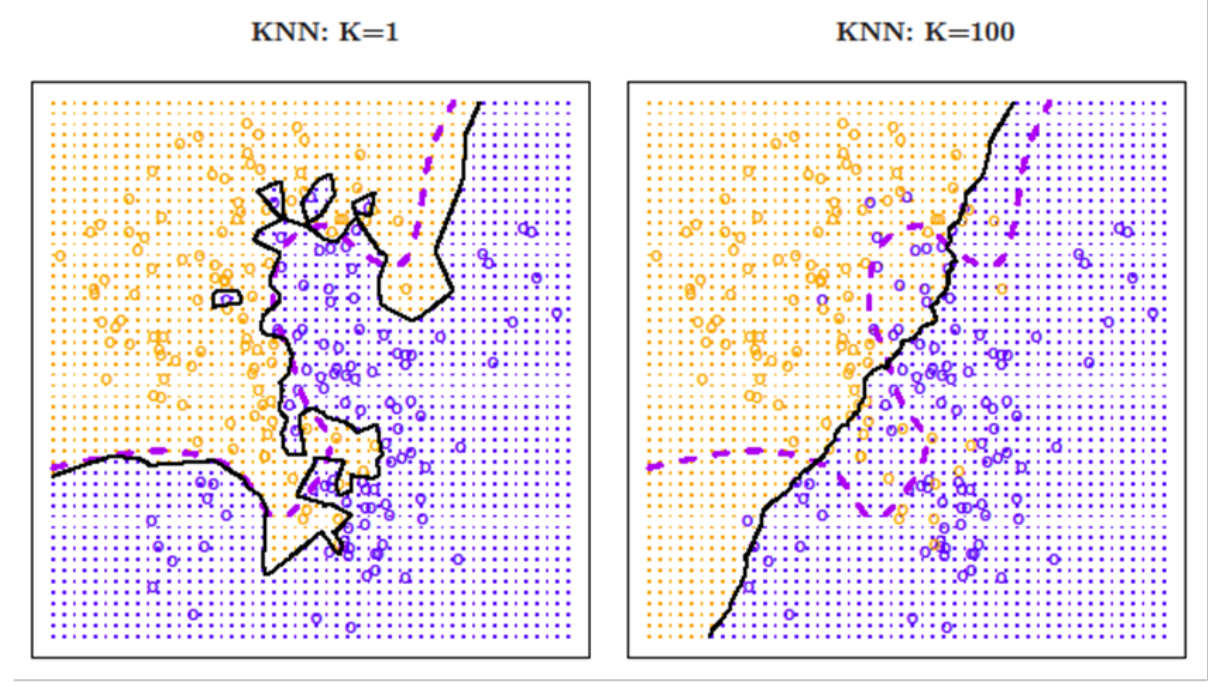
\includegraphics[width=90mm]{figures/knn100}
  \caption{Papel de K en la regularización de KNN}
  \label{fig:knn}
\end{figure}

Podemos observar que un mayor valor de K da lugar a una frontera más
simple, lo que reduce el sobreajuste con el riesgo de que el algoritmo
no sea capaz de ajustarse a los datos de entrenamiento.

Utilizaremos \texttt{KNeighborsClassifier} de \textit{sklearn}, y
probaremos distintos valores (1, 3, 5, 15, 25) para el número de
vecinos más cercanos a considerar (todos impares para evitar empates),
el parámetro \texttt{n\_neighbors} (por defecto 5). Obtenemos los
siguientes resultados: 

\begin{table}[H]
\centering
\caption{Resultados de KNN con distintos valores de K}
\label{tab:knn-tuning}
\begin{tabular}{|lrrrrrrrrrr|}
\hline
 & TP & TN & FP & FN & Acc & TPR & FPR & AUC & F1-score & G-measure\\ \hline
1-NN & 307 & 331 & 94 & 93 & 0.7733 & 0.7675 & 0.2212 & 0.7732 & 0.7665 & 0.7665\\
3-NN & 327 & 345 & 80 & 73 & 0.8145 & 0.8175 & 0.1882 & 0.8146 & 0.8104 & 0.8104\\
5-NN & 324 & 350 & 75 & 76 & 0.817 & 0.81 & 0.1765 & 0.8168 & 0.811 & 0.811\\
15-NN & 328 & 356 & 69 & 72 & 0.8291 & 0.82 & 0.1624 & 0.8288 & 0.8231 & 0.8231\\
25-NN & 325 & 350 & 75 & 75 & 0.8182 & 0.8125 & 0.1765 & 0.818 & 0.8125 & 0.8125\\
\hline
\end{tabular}
\end{table}

Para K=1 obtiene los peores resultados en todas las métricas, esto
probablemente de deba al sobreajuste. Por ejemplo, cualquier dato mal
etiquetado puede provocar que el algoritmo clasifique mal los ejemplos
que caigan en un entorno suyo. Es mucho más difícil que haya 2 o más
datos mal etiquetados cercanos, por lo que el resto de valores de K
obtienen mejores resultados. Los demás valores de K obtienen
resultados similares, pero tomamos K=15, que es el que mejor
puntuación obtiene en las cuatro métricas que consideramos.

\subsection{Red Neuronal}

El último algoritmo que configuramos es la Red Neuronal o Perceptrón
Multicapa. El modelo de Red Neuronal está formado por varias capas,
cada una con varias neuronas, en cada neurona se reciben como entrada
la salida de las neuonas de la capa anterior ponderadas con unos pesos
(que se van entrenando) y se les aplica una función de activación (en
nuestro caso una función \emph{relu}: $f(x)=\max(0,x)$), hasta llegar
a la capa de salida, que devuelve la predicción. Se puede configurar
el número de capas (por defecto: capa de entrada, una capa oculta con
100 neuronas y capa de salida) y el número de neuronas de cada capa,
pero probaremos otra cosa diferente.

Las Redes Neuronales son modelos con gran potencia explicativa, por lo
que tienden al sobreajuste. Probaremos una técnica de regularización
llamada \emph{early stopping}, que aparta una fracción de los datos
(10\% en nuestro caso) para obtener un score de validación. El error
en la muestra de entrenamiento casi seguramente ira a cero, y se
provocará sobreajuste. Esta técnica detiene el entrenamiento cuando el
score de validación no mejora durante un número de iteraciones (10 en
nuestro caso), y ayuda a reducir el sobreajuste. El problema que
podemos tener es nuestro reducido número de datos, no estamos
utilizando una parte de ellos para el entrenamiendo, y puede que el
modelo no aprenda debidamente debido al escaso número de datos. Es por
esto que por defecto no se utiliza esta técnica.

Probamos la implementación de \texttt{MLPClassifier} de
\textit{sklearn} con y sin \texttt{early\_stopping} (también
seleccionamos \texttt{max\_iter=500} porque recibimos un warning de
convergencia). Obtenemos:

\begin{table}[H]
\centering
\caption{Red Neuronal con y sin \emph{early stopping}}
\label{tab:mlp-tuning}
\begin{tabular}{|lrrrrrrrrrr|}
\hline
 & TP & TN & FP & FN & Acc & TPR & FPR & AUC & F1-score & G-measure\\ \hline
RRNN & 333 & 355 & 70 & 67 & 0.8339 & 0.8325 & 0.1647 & 0.8339 & 0.8294 & 0.8294\\
RRNNearly-stopping & 356 & 291 & 134 & 44 & 0.7842 & 0.89 & 0.3153 & 0.7874 & 0.8 & 0.8041\\
\hline
\end{tabular}
\end{table}

Observamos que aplicar esta técnica ha mejorado los aciertos sobre las
instancias positivas, pero al coste de empeorar mucho la clasificación
de instancias negativas. Llega a tener peor F1-score y G-measure, y
mucho peor Acc. y AUC. Es por ello que abandonamos la idea de
\emph{early stopping} y mantenemos la configuración por defecto.

\section{Resultados obtenidos} \label{sec:resultados}

Presentamos los resultados obtenidos por cada uno. Utilizamos los
parámetros por defecto de la implementación de \textit{sklearn} salvo
que se indique lo contrario (para los parámetros que hemos
configurado).

Para los modelos que configuramos en la sección anterior, no mostramos
de nuevo una introducción explicando su funcionamiento. Nos limitamos
a hacerlo para los que no configuramos previamente.

\subsection{\href{https://scikit-learn.org/stable/modules/generated/sklearn.dummy.DummyClassifier.html}{Dummy classifier}}

Es un clasificador que siempre predice un valor constante:
maligno. Obviamente nunca da lugar a falsos negativos, por lo que sus
métricas F1-score y G-measure no son del todo malas. No obstante, es
más que mejorable, ya que no tiene en cuenta las características de
los ejemplos a la hora de clasificarlos. Por tanto lo usamos como cota
inferior: si un algoritmo obtiene peores scores que Dummy, nos
plantearemos si estamos haciendo algo mal o si ese algoritmo es
adecuado para el problema.

El código de creación del modelo es:
\begin{lstlisting}
  dummy=DummyClassifier(strategy='constant',constant=1)
\end{lstlisting}

Sus resultados para cada preprocesado son:

\begin{table}[H]
\centering
\caption{Desempeño de Dummy sobre los distintos preprocesados}
\label{tab:dummy}
\begin{tabular}{|lrrrrrrrrrr|}
\hline
 & TP & TN & FP & FN & Acc & TPR & FPR & AUC & F1-score & G-measure\\ \hline
  Preproc.1 & 400 & 0 & 425 & 0 & 0.4848 & 1.0 & 1.0 & 0.5 & 0.6531 & 0.6963\\
  Preproc.2 & 445 & 0 & 516 & 0 & 0.4631 & 1.0 & 1.0 & 0.5 & 0.633 & 0.6805\\
  Preproc.3 & 400 & 0 & 425 & 0 & 0.4848 & 1.0 & 1.0 & 0.5 & 0.6531 & 0.6963\\
  Preproc.4 & 400 & 0 & 425 & 0 & 0.4848 & 1.0 & 1.0 & 0.5 & 0.6531 & 0.6963\\
  Preproc.5 & 400 & 0 & 425 & 0 & 0.4848 & 1.0 & 1.0 & 0.5 & 0.6531 & 0.6963\\
\hline
\end{tabular}
\end{table}

\subsection{\href{https://scikit-learn.org/stable/modules/generated/sklearn.tree.DecisionTreeClassifier.html}{Árbol de decisión}}

Como explicamos previamente, limitamos la profundidad del árbol a 3
nodos. El resto de parámetros son los elegidos por defecto en la
implementación.

El código de creación del modelo es:
\begin{lstlisting}
  dt=tree.DecisionTreeClassifier(max_depth=3,random_state=SEED)
\end{lstlisting}

Sus resultados para cada preprocesado son:

\begin{table}[H]
\centering
\caption{Desempeño de Decision Tree sobre los distintos preprocesados}
\label{tab:dt}
\begin{tabular}{|lrrrrrrrrrr|}
\hline
 & TP & TN & FP & FN & Acc & TPR & FPR & AUC & F1-score & G-measure\\ \hline
  Preproc.1 & 308 & 380 & 45 & 92 & 0.8339 & 0.77 & 0.1059 & 0.8321 & 0.8181 & 0.8197\\
  Preproc.2 & 337 & 458 & 58 & 108 & 0.8273 & 0.7573 & 0.1124 & 0.8225 & 0.8024 & 0.8038\\
  Preproc.3 & 309 & 380 & 45 & 91 & 0.8352 & 0.7725 & 0.1059 & 0.8333 & 0.8196 & 0.8212\\
  Preproc.4 & 308 & 382 & 43 & 92 & 0.8364 & 0.77 & 0.1012 & 0.8344 & 0.8202 & 0.822\\
  Preproc.5 & 308 & 382 & 43 & 92 & 0.8364 & 0.77 & 0.1012 & 0.8344 & 0.8202 & 0.822\\
\hline
\end{tabular}
\end{table}

\subsection{\href{https://scikit-learn.org/stable/modules/generated/sklearn.ensemble.RandomForestClassifier.html}{Random Forest}}

Seleccionamos 1000 estimadores simples, utilizamos \texttt{n\_jobs=4}
para paralelizar el cómputo. El resto de parámetros son los elegidos
por defecto en la implementación.

El código de creación del modelo es:
\begin{lstlisting}
  rf=RandomForestClassifier(n_estimators=1000, n_jobs=4, random_state=SEED)
\end{lstlisting}

Sus resultados para cada preprocesado son:

\begin{table}[H]
\centering
\caption{Desempeño de Random Forest sobre los distintos preprocesados}
\label{tab:rf}
\begin{tabular}{|lrrrrrrrrrr|}
\hline
 & TP & TN & FP & FN & Acc & TPR & FPR & AUC & F1-score & G-measure\\ \hline
  Preproc.1 & 322 & 347 & 78 & 78 & 0.8109 & 0.805 & 0.1835 & 0.8107 & 0.805 & 0.805\\
  Preproc.2 & 344 & 419 & 97 & 101 & 0.794 & 0.773 & 0.188 & 0.7925 & 0.7765 & 0.7765\\
  Preproc.3 & 322 & 344 & 81 & 78 & 0.8073 & 0.805 & 0.1906 & 0.8072 & 0.802 & 0.802\\
  Preproc.4 & 325 & 340 & 85 & 75 & 0.8061 & 0.8125 & 0.2 & 0.8063 & 0.8025 & 0.8025\\
  Preproc.5 & 327 & 339 & 86 & 73 & 0.8073 & 0.8175 & 0.2024 & 0.8076 & 0.8044 & 0.8045\\
\hline
\end{tabular}
\end{table}

\subsection{\href{https://scikit-learn.org/stable/modules/generated/sklearn.svm.SVC.html}{Support Vector Machine}}

Regularizamos con \texttt{C=0.25}. El resto de parámetros son los
elegidos por defecto en la implementación.

El código de creación del modelo es:
\begin{lstlisting}
  svc=SVC(C=0.25, random_state=SEED)
\end{lstlisting}

Sus resultados para cada preprocesado son:

\begin{table}[H]
\centering
\caption{Desempeño de SVM sobre los distintos preprocesados}
\label{tab:svm}
\begin{tabular}{|lrrrrrrrrrr|}
\hline
 & TP & TN & FP & FN & Acc & TPR & FPR & AUC & F1-score & G-measure\\ \hline
  Preproc.1 & 297 & 298 & 127 & 103 & 0.7212 & 0.7425 & 0.2988 & 0.7218 & 0.7209 & 0.7212\\
  Preproc.2 & 298 & 381 & 135 & 147 & 0.7066 & 0.6697 & 0.2616 & 0.704 & 0.6788 & 0.6789\\
  Preproc.3 & 296 & 299 & 126 & 104 & 0.7212 & 0.74 & 0.2965 & 0.7218 & 0.7202 & 0.7205\\
  Preproc.4 & 278 & 292 & 133 & 122 & 0.6909 & 0.695 & 0.3129 & 0.691 & 0.6856 & 0.6856\\
  Preproc.5 & 344 & 351 & 74 & 56 & 0.8424 & 0.86 & 0.1741 & 0.8429 & 0.8411 & 0.8413\\
\hline
\end{tabular}
\end{table}

\subsection{\href{https://scikit-learn.org/stable/modules/generated/sklearn.naive_bayes.GaussianNB.html}{Gaussian Naive-Bayes}}
Este modelo se basa en el
\href{https://en.wikipedia.org/wiki/Bayes%27_theorem}{Teorema de Bayes}
  para la estimación de la probabilidad de que una instancia
  pertenezca una determinada a clase dado un valor de una variable
  utilizando la probabilidad de que la variable presente ese valor si
  la instancia pertenece a la anterior clase. Esta última probabilidad
  se estima usando las frecuencias relativas en el caso de variables
  discretas, para las variables numéricas se supone que se distribuyen
  por una normal (de ahí el nombre de Gaussian). También se supone que
  las variables son independientes, por lo que este modelo puede
  beneficiarse de la eliminación de características redundantes o
  innecesarias.

El código de creación del modelo es:
\begin{lstlisting}
  gnb=GaussianNB()
\end{lstlisting}

Sus resultados para cada preprocesado son:

\begin{table}[H]
\centering
\caption{Desempeño de Naive-Bayes sobre los distintos preprocesados}
\label{tab:gnb}
\begin{tabular}{|lrrrrrrrrrr|}
\hline
 & TP & TN & FP & FN & Acc & TPR & FPR & AUC & F1-score & G-measure\\ \hline
  Preproc.1 & 341 & 340 & 85 & 59 & 0.8255 & 0.8525 & 0.2 & 0.8263 & 0.8257 & 0.8261\\
  Preproc.2 & 374 & 413 & 103 & 71 & 0.8189 & 0.8404 & 0.1996 & 0.8204 & 0.8113 & 0.8118\\
  Preproc.3 & 346 & 347 & 78 & 54 & 0.84 & 0.865 & 0.1835 & 0.8407 & 0.8398 & 0.8402\\
  Preproc.4 & 354 & 321 & 104 & 46 & 0.8182 & 0.885 & 0.2447 & 0.8201 & 0.8252 & 0.8271\\
  Preproc.5 & 354 & 321 & 104 & 46 & 0.8182 & 0.885 & 0.2447 & 0.8201 & 0.8252 & 0.8271\\
\hline
\end{tabular}
\end{table}

\subsection{\href{https://scikit-learn.org/stable/modules/generated/sklearn.neighbors.KNeighborsClassifier.html}{KNN}}

Elegimos tener en cuenta los 15 vecinos más cercanos. El resto de
parámetros son los elegidos por defecto en la implementación.

El código de creación del modelo es:
\begin{lstlisting}
  knn=KNeighborsClassifier(n_neighbors=15)
\end{lstlisting}

Sus resultados para cada preprocesado son:

\begin{table}[H]
\centering
\caption{Desempeño de KNN sobre los distintos preprocesados}
\label{tab:knn}
\begin{tabular}{|lrrrrrrrrrr|}
\hline
 & TP & TN & FP & FN & Acc & TPR & FPR & AUC & F1-score & G-measure\\ \hline
  Preproc.1 & 338 & 317 & 108 & 62 & 0.7939 & 0.845 & 0.2541 & 0.7954 & 0.7991 & 0.8002\\
  Preproc.2 & 368 & 399 & 117 & 77 & 0.7981 & 0.827 & 0.2267 & 0.8001 & 0.7914 & 0.7921\\
  Preproc.3 & 341 & 311 & 114 & 59 & 0.7903 & 0.8525 & 0.2682 & 0.7921 & 0.7977 & 0.7993\\
  Preproc.4 & 329 & 331 & 94 & 71 & 0.8 & 0.8225 & 0.2212 & 0.8007 & 0.7995 & 0.7998\\
  Preproc.5 & 328 & 356 & 69 & 72 & 0.8291 & 0.82 & 0.1624 & 0.8288 & 0.8231 & 0.8231\\
\hline
\end{tabular}
\end{table}

\subsection{\href{https://scikit-learn.org/stable/modules/generated/sklearn.neural_network.MLPClassifier.html}{Red neuronal}}

Mantuvimos la configuración por defecto, porque los resultados de
\emph{early stopping} no fueron satisfactorios. Seleccionamos
\texttt{max\_iter=500} porque con el valor por defecto (200)
recibíamos un warning de convergencia.

El código de creación del modelo es:
\begin{lstlisting}
  rn=MLPClassifier(max_iter=500,random_state=SEED)
\end{lstlisting}

Sus resultados para cada preprocesado son:

\begin{table}[H]
\centering
\caption{Desempeño de la Red Neuronal sobre los distintos preprocesados}
\label{tab:mlp}
\begin{tabular}{|lrrrrrrrrrr|}
\hline
 & TP & TN & FP & FN & Acc & TPR & FPR & AUC & F1-score & G-measure\\ \hline
  Preproc.1 & 337 & 332 & 93 & 63 & 0.8109 & 0.8425 & 0.2188 & 0.8118 & 0.812 & 0.8126\\
  Preproc.2 & 366 & 410 & 106 & 79 & 0.8075 & 0.8225 & 0.2054 & 0.8085 & 0.7983 & 0.7986\\
  Preproc.3 & 323 & 338 & 87 & 77 & 0.8012 & 0.8075 & 0.2047 & 0.8014 & 0.7975 & 0.7976\\
  Preproc.4 & 342 & 337 & 88 & 58 & 0.823 & 0.855 & 0.2071 & 0.824 & 0.8241 & 0.8246\\
  Preproc.5 & 333 & 355 & 70 & 67 & 0.8339 & 0.8325 & 0.1647 & 0.8339 & 0.8294 & 0.8294\\
\hline
\end{tabular}
\end{table}

\section{Análisis de resultados} \label{sec:analisis}

Sobre cada uno de los preprocesamientos, discutiremos el desempeño de
los modelos configurados y cuál es el más adecuado para el problema.
Comenzaremos con una comparación general, y para cada preprocesamiento
nos centraremos en qué ha cambiado e intentaremos buscar
explicaciones.

\subsection{Sobre preprocesado 1: Eliminación de valores perdidos}

\begin{table}[H]
\centering
\caption{Resultados de los algoritmos configurados al eliminar los
  datos con valores perdidos}
\label{tab:res-dropna}
\begin{tabular}{|lrrrrrrrrrr|}
\hline
 & TP & TN & FP & FN & Acc & TPR & FPR & AUC & F1-score & G-measure\\ \hline
Dummy & 400 & 0 & 425 & 0 & 0.4848 & 1.0 & 1.0 & 0.5 & 0.6531 & 0.6963\\
DecisionTree & 308 & 380 & 45 & 92 & 0.8339 & 0.77 & 0.1059 & 0.8321 & 0.8181 & 0.8197\\
GaussianNB & 341 & 340 & 85 & 59 & 0.8255 & 0.8525 & 0.2 & 0.8263 & 0.8257 & 0.8261\\
SupportVectorM & 297 & 298 & 127 & 103 & 0.7212 & 0.7425 & 0.2988 & 0.7218 & 0.7209 & 0.7212\\
RandomForest & 322 & 347 & 78 & 78 & 0.8109 & 0.805 & 0.1835 & 0.8107 & 0.805 & 0.805\\
KNN & 338 & 317 & 108 & 62 & 0.7939 & 0.845 & 0.2541 & 0.7954 & 0.7991 & 0.8002\\
NeuralNetwork & 337 & 332 & 93 & 63 & 0.8109 & 0.8425 & 0.2188 & 0.8118 & 0.812 & 0.8126\\
\hline
\end{tabular}
\end{table}

Atendiendo a Acc. y AUC, el modelo que mejores resultados obtiene es
Árbol de Decisión, seguido por Naive-Bayes y el resto de modelos
excepto SVM, que se queda bastante atrás. Todos los modelos, incluso
SVM, superan con creces a Dummy.

Atendiendo a las métricas F1-score y G-measure, ocurre algo similar,
con la excepción de que esta vez es Naive-Bayes el algoritmo que
consigue los máximos scores, ya que el Árbol de decisión falla más al
clasificar los ejemplos positivos y estas métricas los priorizan más.

Podemos utilizar las métricas TPR (proporción de instancias positivas
bien clasificadas) y FPR (proporción de instancias negativas mal
clasificadas) para representar los modelos en el espacio ROC,
recordemos que un modelo es mejor si en el espacio ROC se sitúa más al
noroeste.

\begin{figure}[H]
  \centering
  \label{fig:roc1}
  \caption{Algoritmos sobre el preprocesado 1 representados en el espacio ROC}
  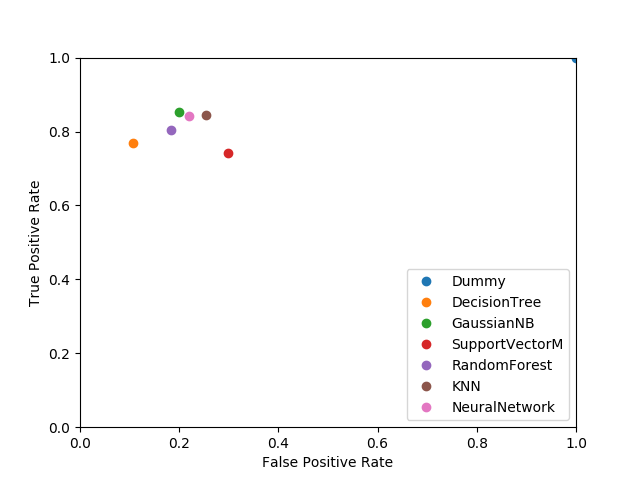
\includegraphics[width=80mm]{figures/roc1}
\end{figure}

Observamos que Naive-Bayes obtiene mejores resultados que la mayoría
de modelos, se ve superado por el Árbol de Decisión en la
clasificación de elementos negativos (DecisionTree está mas al oeste),
pero a la hora de clasificar positivos tiene más éxito Naive-Bayes
(está más al norte), lo que refleja sus mejores F1-score y G-measure.

\subsection{Sobre preprocesado 2: Imputación de valores perdidos}
Como dijimos en su momento, sólo consideraremos la mediana para
imputar valores perdidos en variables numéricas, ya que obtuvo mejores
resultados que la media.

\begin{table}[H]
\centering
\caption{Resultados de los algoritmos configurados al imputar las
  variables numéricas con la mediana y las nominales con la moda}
\label{tab:res-median}
\begin{tabular}{|lrrrrrrrrrr|}
\hline
 & TP & TN & FP & FN & Acc & TPR & FPR & AUC & F1-score & G-measure\\ \hline
Dummy & 445 & 0 & 516 & 0 & 0.4631 & 1.0 & 1.0 & 0.5 & 0.633 & 0.6805\\
DecisionTree & 337 & 458 & 58 & 108 & 0.8273 & 0.7573 & 0.1124 & 0.8225 & 0.8024 & 0.8038\\
GaussianNB & 374 & 413 & 103 & 71 & 0.8189 & 0.8404 & 0.1996 & 0.8204 & 0.8113 & 0.8118\\
SupportVectorM & 298 & 381 & 135 & 147 & 0.7066 & 0.6697 & 0.2616 & 0.704 & 0.6788 & 0.6789\\
RandomForest & 344 & 419 & 97 & 101 & 0.794 & 0.773 & 0.188 & 0.7925 & 0.7765 & 0.7765\\
KNN & 368 & 399 & 117 & 77 & 0.7981 & 0.827 & 0.2267 & 0.8001 & 0.7914 & 0.7921\\
NeuralNetwork & 366 & 410 & 106 & 79 & 0.8075 & 0.8225 & 0.2054 & 0.8085 & 0.7983 & 0.7986\\
\hline
\end{tabular}
\end{table}

Observamos que todos los modelos han visto minada su capacidad de
predicción en las cuatro métricas que estamos considerando, excepto
KNN con las métricas Acc. y AUC, que han aumentado levemente. Pero
aunque haya clasificado bien más ejemplos, ha perdido eficacia a la
hora de clasificar ejemplos positivos, por lo que las métricas
F1-score y G-measure han empeorado. Es por esto que abandonamos en su
momento la idea de imputar los valores perdidos.

\begin{figure}[H]
  \centering
  \label{fig:roc2}
  \caption{Algoritmos sobre el preprocesado 2 representados en el espacio ROC}
  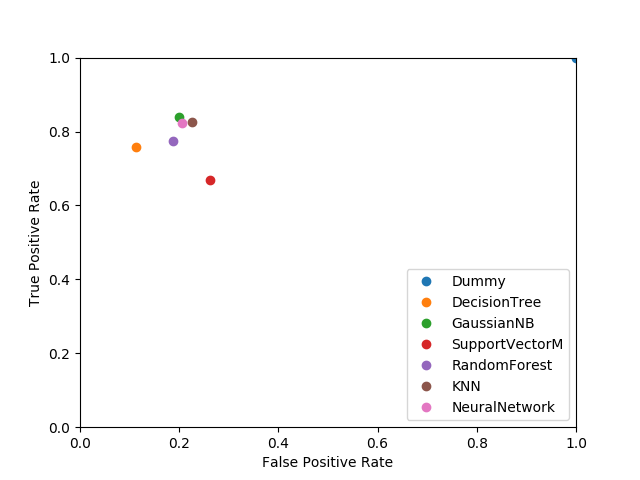
\includegraphics[width=80mm]{figures/roc2}
\end{figure}

En el espacio ROC, imputar los valores perdidos no ha provocado que
algún modelo sobrepase a otro, simplemente han empeorado en distinta
medida sus scores.

\subsection{Sobre preprocesado 3: Eliminación de características
  innecesarias}

La simplificación del conjunto de características se realiza sobre los
datos sin las instancias con valores perdidos, es por eso que debemos
comparar esta tabla con la Tabla \ref{tab:res-dropna}.

\begin{table}[H]
\centering
\caption{Resultados de los algoritmos configurados al simplificar el
  conjunto de características}
\label{tab:res-features}
\begin{tabular}{|lrrrrrrrrrr|}
\hline
 & TP & TN & FP & FN & Acc & TPR & FPR & AUC & F1-score & G-measure\\ \hline
Dummy & 400 & 0 & 425 & 0 & 0.4848 & 1.0 & 1.0 & 0.5 & 0.6531 & 0.6963\\
DecisionTree & 309 & 380 & 45 & 91 & 0.8352 & 0.7725 & 0.1059 & 0.8333 & 0.8196 & 0.8212\\
GaussianNB & 346 & 347 & 78 & 54 & 0.84 & 0.865 & 0.1835 & 0.8407 & 0.8398 & 0.8402\\
SupportVectorM & 296 & 299 & 126 & 104 & 0.7212 & 0.74 & 0.2965 & 0.7218 & 0.7202 & 0.7205\\
RandomForest & 322 & 344 & 81 & 78 & 0.8073 & 0.805 & 0.1906 & 0.8072 & 0.802 & 0.802\\
KNN & 341 & 311 & 114 & 59 & 0.7903 & 0.8525 & 0.2682 & 0.7921 & 0.7977 & 0.7993\\
NeuralNetwork & 323 & 338 & 87 & 77 & 0.8012 & 0.8075 & 0.2047 & 0.8014 & 0.7975 & 0.7976\\
\hline
\end{tabular}
\end{table}

Esta vez sí observamos comportamientos distintos entre modelos.
Observamos un aumento en la mayoría de modelos en las cuatro métricas
que consideramos, con la excepción de la Red Neuronal, que parecía
aprovechar parte de la información que hemos desechado y por tanto ha
bajado. En el caso de Naive-Bayes, se ha producido una mejora
significativa, esto se debe a que al simplificar el conjunto de
variables es probable que disminuya el grado de dependencia entre las
mismas, por lo que la suposición que realiza este modelo de que las
características son independientes cobra más realismo.

\begin{figure}[H]
  \centering
  \label{fig:roc3}
  \caption{Algoritmos sobre el preprocesado 3 representados en el espacio ROC}
  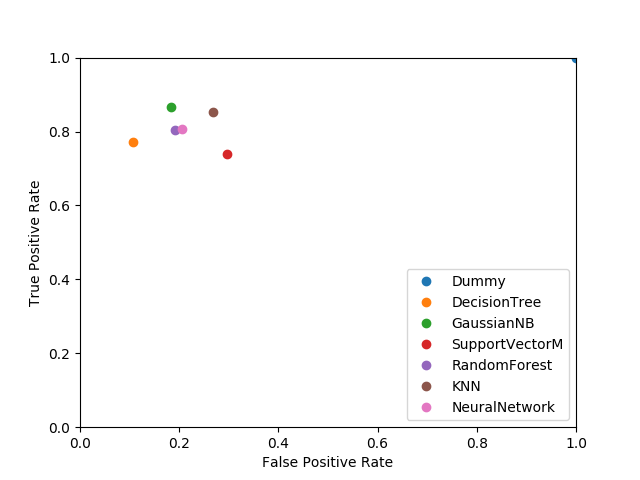
\includegraphics[width=80mm]{figures/roc3}
\end{figure}

GaussianNB ahora sobrepasa a Random Forest a la hora de clasificar
elementos negativos (se sitúa más al oeste), y ya es mejor que
cualquiera de los demás modelos salvo el Árbol de decisión, pero éste
clasifica bastante mal los positivos en comparación con el resto, sólo
supera a Naive-Bayes a la hora de clasificar negativos, por lo que sus
métricas F1-score y G-measure son bastante peores.

\subsection{Sobre preprocesado 4: Binarización de características
  nominales}

La binarización se produce sobre los datos del preprocesado 3, así que
debemos comparar esta tabla con la Tabla \ref{tab:res-features}.

\begin{table}[H]
\centering
\caption{Resultados de los algoritmos configurados al binarizar las características nominales}
\label{tab:res-binarization}
\begin{tabular}{|lrrrrrrrrrr|}
\hline
 & TP & TN & FP & FN & Acc & TPR & FPR & AUC & F1-score & G-measure\\ \hline
Dummy & 400 & 0 & 425 & 0 & 0.4848 & 1.0 & 1.0 & 0.5 & 0.6531 & 0.6963\\
DecisionTree & 308 & 382 & 43 & 92 & 0.8364 & 0.77 & 0.1012 & 0.8344 & 0.8202 & 0.822\\
GaussianNB & 354 & 321 & 104 & 46 & 0.8182 & 0.885 & 0.2447 & 0.8201 & 0.8252 & 0.8271\\
SupportVectorM & 278 & 292 & 133 & 122 & 0.6909 & 0.695 & 0.3129 & 0.691 & 0.6856 & 0.6856\\
RandomForest & 325 & 340 & 85 & 75 & 0.8061 & 0.8125 & 0.2 & 0.8063 & 0.8025 & 0.8025\\
KNN & 329 & 331 & 94 & 71 & 0.8 & 0.8225 & 0.2212 & 0.8007 & 0.7995 & 0.7998\\
NeuralNetwork & 342 & 337 & 88 & 58 & 0.823 & 0.855 & 0.2071 & 0.824 & 0.8241 & 0.8246\\
\hline
\end{tabular}
\end{table}

Este preprocesado ha provocado una mejora significativa en la Red
Neuronal, que parece aprovecharse de que el número de variables sea
alto.

Cuando introdujimos esta idea, comentamos porqué KNN debía
beneficiarse de ella, sin embargo la mejora de sus resultados es
bastante leve, y se debe a un aumento de aciertos en elementos de la
clase negativa (de hecho los aciertos en positivos decrecen), por lo
que apenas cambian las métricas F1-score y G-measure.

Naive-Bayes ha vuelto a bajar, debido a que estamos introduciendo más
características que por supuesto no son independientes. Por ejemplo,
al eliminar Margin introducimos 5 variables binarias, y el hecho de
que alguna de ellas valga 1 obliga a las otras 4 a valer 0, por lo que
son muy bastante dependientes.

En cuanto a SVM, sufre una caída significativa en todos sus scores.
Viendo su posterior desempeño tras el preprocesamiento 5, sospechamos
que éste algoritmo requiere que las variables presenten escalas
similares, y convertir variables que toman valores entre 1 y 4 o entre
1 y 5 en variables que toman los valores 0 y 1, aumenta aun más la
diferencia de escala con la variable Age.

El resto de modelos apenas experimentan cambios en sus scores.

\begin{figure}[H]
  \centering
  \label{fig:roc4}
  \caption{Algoritmos sobre el preprocesado 4 representados en el espacio ROC}
  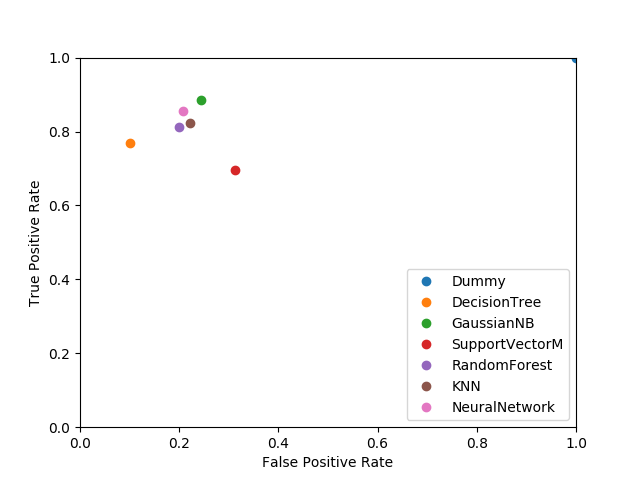
\includegraphics[width=80mm]{figures/roc4}
\end{figure}

En el espacio ROC, los modelos Neural Network, KNN y Random Forest
sobrepasan a Naive-Bayes a la hora de clasificar ejemploso negativos,
pero NB sigue siendo el que mejor clasifica los positivos, que para
nuestro problema tienen prioridad.

\subsection{Sobre preprocesado 5: Reescalado de los datos}

Comparamos esta tabla con la tabla \ref{tab:res-binarization}.

\begin{table}[H]
\centering
\caption{Resultados de los algoritmos configurados al estandarizar las
  variables}
\label{tab:res-stdScaler}
\begin{tabular}{|lrrrrrrrrrr|}
\hline
 & TP & TN & FP & FN & Acc & TPR & FPR & AUC & F1-score & G-measure\\ \hline
Dummy & 400 & 0 & 425 & 0 & 0.4848 & 1.0 & 1.0 & 0.5 & 0.6531 & 0.6963\\
DecisionTree & 308 & 382 & 43 & 92 & 0.8364 & 0.77 & 0.1012 & 0.8344 & 0.8202 & 0.822\\
GaussianNB & 354 & 321 & 104 & 46 & 0.8182 & 0.885 & 0.2447 & 0.8201 & 0.8252 & 0.8271\\
SupportVectorM & 344 & 351 & 74 & 56 & 0.8424 & 0.86 & 0.1741 & 0.8429 & 0.8411 & 0.8413\\
RandomForest & 327 & 339 & 86 & 73 & 0.8073 & 0.8175 & 0.2024 & 0.8076 & 0.8044 & 0.8045\\
KNN & 328 & 356 & 69 & 72 & 0.8291 & 0.82 & 0.1624 & 0.8288 & 0.8231 & 0.8231\\
NeuralNetwork & 333 & 355 & 70 & 67 & 0.8339 & 0.8325 & 0.1647 & 0.8339 & 0.8294 & 0.8294\\
\hline
\end{tabular}
\end{table}

Al estandarizar los atributos, los árboles tienen idéntico
comportamiento porque ellos tratan las variables por separado (en cada
nodo toman una decisión de acuerdo a una única característica). Lo
mismo le ocurre a GaussianNB, que supone las variables independientes
y no atiende a las relaciones entre las mismas.

KNN se beneficia bastante de esta medida, ya que le estaba dando una
importancia exagerada a la Edad, que presentaba una escala mucho mayor
que el resto de variables.

Neural Network también experimenta una leve mejora, el hecho de que
las características presenten escalas similares acostumbra a facilitar
el aprendizaje de modelos de este tipo.

El gran beneficiado con esta técnica es SVM, que parece depender
fuertemente de que las escalas de las variables sean similares. Ha
obtenido los mejores scores en las cuatro métricas que estamos
considerando.

\begin{figure}[H]
  \centering
  \label{fig:roc5}
  \caption{Algoritmos sobre el preprocesado 5 representados en el espacio ROC}
  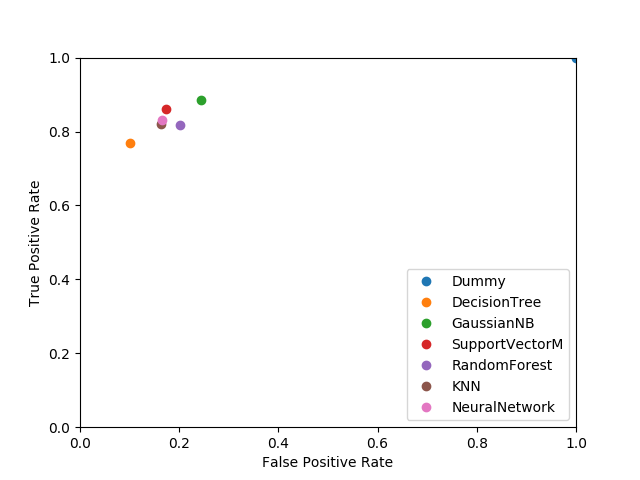
\includegraphics[width=80mm]{figures/roc5}
\end{figure}

En el espacio ROC, SVM sobrepasa a todos los modelos excepto a
Naive-Bayes a la hora de clasificar instancias positivas, pero su
mucho mayor éxito con las instancias negativas compensa.

Consideramos que SVM con el procesamiento 5 es el más adecuado para el
problema. Suponiendo que F1-score y G-measure son métricas adecuadas
para lograr un equilibrio entre priorizar los aciertos en las clases
positivas y el desempeño general de los algoritmos.

\subsection{¿Qué podríamos mejorar?}

Para intentar mejorar los resultados, podríamos intentar algunos
cambios más tanto en la configuración de los modelos como en el
preprocesado de datos.

En el caso de SVM, que ha conseguido los mejores resultados (con el
preprocesado 5), podríamos experimentar con diferentes kernels, como
polinomios de distintos grados, lineal, sigmoide, etc. También
podríamos ajustar con más precisión el parámetro de regularización C,
probando una amplia gama de valores alrededor de 0.25.

Naive-Bayes también ha conseguido muy buenos resultados con el
preprocesado 3, pero fue perjudicado por el preprocesado 4. Podríamos
no realizar el preprocesado 4 e intentar otras técnicas de
preprocesado como las que detallamos más adelante.

En el caso de Decision Tree, una posibilidad sería cambiar de criterio
para elegir por qué variable separar en cada nodo. Además de Gini, la
entropía es otro criterio muy utilizado que no hemos probado
(algoritmo ID3).

Random Forest es un modelo muy flexible y con muchos parámetros,
podríamos intentar cambiar más parámetros como son el criterio para
medir la calidad de la separación en un nodo (por defecto usa Gini,
podríamos probar Entropy), la profundidad máxima de los estimadores
(para el Árbol de Decisión, ha dado muy buenos resultados) o la
cantidad de muestras/variables que se utilizan para construir los
estimadores simples (por defecto se utilizan todas las muestras y la
raíz cuadrada del número de variables, para esto último también se
suele utilizar el logaritmo en base dos del número de datos).

También en los árboles, se puede introducir un parámetro $\alpha$,
quepenaliza el número de nodos del árbol, con el objetivo de
regularizar y obtener árboles más simples.

Para KNN, podríamos haber experimentado con otras métricas en lugar de
la euclídea como la
\href{https://en.wikipedia.org/wiki/Taxicab_geometry}{distancia
  Manhattan} o la
\href{https://en.wikipedia.org/wiki/Uniform_norm}{norma del máximo},
también podríamos haberle dado más peso a los vecinos más cercanos
(dentro de los 15 que se tienen en cuenta, que el voto de cada uno
tenga un peso inversamente proporcional a la distancia a la que se
encuentra). También podríamos haber probado una gama más amplia de
valores de K.

Para la Red Neuronal, podríamos haber intentado distintas
arquitecturas jugando con el número de capas y el número de neuronas
de cada una. También podríamos haber probado con distintas funciones
de activación (en lugar de relu que es la por defecto, sigmoide o
tangente hiperbólica). También se puede ajustar un parámetro de
regularización $\alpha$ para penalizar los pesos elevados.

Para el preprocesamiento, podríamos haber estudiado otras formas de
imputar los valores perdidos, ya que las que hemos probado no han dado
buen resultado. Con \texttt{KNNImputer} de \textit{sklearn}, podemos
usar la técnica de los K vecinos más cercanos para imputar valores
perdidos. También existen otras técnicas como las basadas en SVM.

\section{Interpretación de resultados} \label{sec:interpretacion}

Analizaremos dos modelos para determinar los factores que más
contribuyen a la pertenencia a una determinada clase. Ambos modelos
utilizan árboles, así que los ejecutaremos sobre el preprocesado 4,
que produce el mismo comportamiento que el 5.

\subsection{Visualización del Árbol de Decisión}
Visualizaremos el Árbol de Decisión obtenido, cuya profundidad
limitamos a 3. Esto nos permite conocer las reglas de clasificación
que utiliza el modelo con un simple vistazo.

\begin{figure}[H]
  \centering
  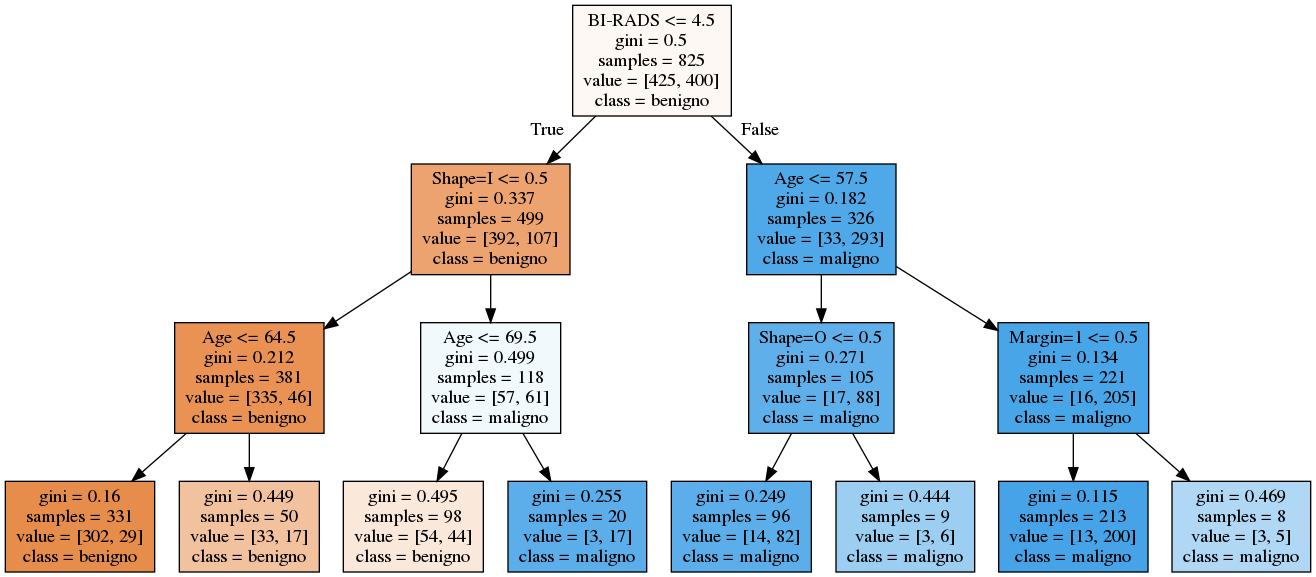
\includegraphics[width=190mm]{figures/tree}
  \caption{Árbol de Decisión}
  \label{fig:tree}
\end{figure}

Observamos que cuando el código BI-RADS es mayor o igual a 4.5 (es
decir, 5 ó 6, que colapsamos a 5), el árbol automáticamente predice
que el tumor es maligno. Para código BI-RADS 4 o menor (que colapsamos
a 4), siempre predice benigno salvo que la forma sea Irregular y el
paciente sea mayor de 69 años, que predice maligno.

Por ejemplo, si una instancia presenta código BI-RADS 4, cae en el
subárbol de la izquierda, y si la forma del tumor no fuese Irregular,
volvería a caer hacia la izquierda. Según la edad del paciente, caería
en el nodo hoja de más a la izquierda o en el segundo, pero igualmente
se catalogaría como benigno.

Observamos que la variable que más ayuda a decididir a este modelo es
el código BI-RADS, lo que lo convierte en un factor clave a la hora de
realizar la predicción.

\subsection{Importancia de las características para Random Forest}

Podemos pedir a Random Forest que asigne un porcentaje de importancia
a las características según la frecuencia con la que aparecen en los
niveles altos de los árboles que utiliza como clasificadores simples.
Recordemos que el desempeño de Random Forest ha sido algo peor que el
del Árbol de Decisión.

Conseguimos esto con el atributo \texttt{feature\_importances\_} de la
clase \texttt{RandomForestClassifier}, con el modelo ya entrenado.

La importancia de las características que hemos obtenido es:

\begin{table}[H]
  \centering
  \begin{tabular}{r|l}
    Age & 0.3615 \\
    BI-RADS & 0.2813 \\
    Margin=1 & 0.1378 \\
    Shape=I & 0.1027 \\
    Shape=O & 0.03 \\
    Shape=R & 0.0242 \\
    Margin=4 & 0.0192 \\
    Margin=5 & 0.0168 \\
    Shape=L & 0.0114 \\
    Margin=3 & 0.0098 \\
    Margin=2 & 0.0055 \\
  \end{tabular}
  \caption{Importancia de las variables asignada por Random Forest}
  \label{tab:importance}
\end{table}

La característica que más utiliza Random Forest para separar los datos
de un nodo es la edad, tampoco debe sorprendernos, puesto que tiene un
rango de valores mucho más amplio que el resto de variables (que solo
pueden tomar dos valores). También se basa bastante el código BI-RADS,
como cabría esperar.

El hecho de que la forma de la masa tumoral sea Irregular, es el la
segunda tercera característica más importante, esto concuerda con su
aparición en el hijo izquierdo de la raíz en el árbol de decisión. Le
sigue comprobar si el margen vale 1 (circumscribed), que aparece en el
nodo más a la derecha del nivel 2 (empezando en 0) del árbol de
decisión. Y bastante por detrás, comprobar si la forma es Ovalada,
queaparece en el nodo de la izquierda del antes mencionado.

Podemos sumar las características binarias en las que hemos desplegado
Margin y Shape para tener una idea de la importancia de estas
características.

\begin{table}[H]
  \centering
  \begin{tabular}{r|l}
    Age & 0.3615 \\
    BI-RADS & 0.2813 \\
    Margin & 0.189 \\
    Shape & 0.1682 \\
  \end{tabular}
  \caption{Importancia de las variables asignada por Random Forest, agrupando Shape y Margin}
  \label{tab:importance2}
\end{table}

Y parece que Margin ha tenido más relevancia para Random Foreset, pero
ambas siguen por debajo de Age y BI-RADS.

Ahora podríamos preguntarnos, ¿qué hubiese pasado si no hubiesemos
simplificado el conjuto de características? Volvemos a hacer esto,
pero manteniendo la distribución original de BI-RADS (sin colapsar
valores) y la columna Density (que eliminamos). También omitimos la
binarización de características nominales, ya que para los árboles no
suele ser un problema trabajar con ellas. Esta vez obtenemos:

\begin{table}[H]
  \centering
  \begin{tabular}{r|l}
    BI-RADS & 0.3266 \\
    Age & 0.311 \\
    Margin & 0.1788 \\
    Shape & 0.1563 \\
    Density & 0.0273 \\
  \end{tabular}
  \caption{Importancia de las variables asignada por Random Forest, sobre procesamiento básico}
  \label{tab:importance3}
\end{table}

Efectivamente la relevancia de Density a la hora de clasificar las
muestras es muy baja, por lo que hicimos bien eliminándola. Aunque
parece que simplificar los valores de BI-RADS (colapsando en 4 y 5)
provocó que la variable perdiese interés y se viese superada por Age
en importancia para Random Forest. Repetimos este experimento, pero
esta vez mantenemos simplificados los valores de BI-RADS.

\begin{table}[H]
  \centering
  \begin{tabular}{r|l}
    Age & 0.3219 \\
    BI-RADS & 0.3153 \\
    Margin & 0.1798 \\
    Shape & 0.1558 \\
    Density & 0.0272 \\
  \end{tabular}
  \caption{Importancia de las variables asignada por Random Forest, manteniendo Density pero simplificando BI-RADS}
  \label{tab:importance4}
\end{table}

Efectivamente su simplificación le hizo perder a la variable BI-RADS
algo de importancia. Pero la mayor pérdida de importancia de BI-RADS
se produce cuando eliminamos Density. Por tanto esta decisión (de
simplificar los valores de BI-RADS) no ha tenido demasiada repercusión
respecto al interés de la variable.

\section{Contenido adicional}

\subsection{Disposición de los datos}

En la sección \ref{sec:configuracion} vemos en algunos modelos que a
mayor regularización sube TP (elementos positivos clasificados
correctamente) pero baja TN (elementos negativos clasificados
correctamente). Esto se observa en las regularizaciones de los
algoritmos:

\begin{itemize}
\item Random Forest, Tablas \ref{tab:rf-tuning} y
  \ref{tab:rf-tuning2}: Al aumentar el número de estimadores decrece
  la dependencia de los datos de entrenamiento.
\item SVM, Tabla \ref{tab:svm-tuning}: Un valor menor de C da lugar a
  una frontera con mayor margen, aunque permite que algunos valores
  los violen. C=50 es una excepción de esta regla.
\item Neural Network, Tabla \ref{tab:mlp-tuning}: Regularizar con
  \emph{early stopping} provoca una mejor clasificación de las
  instancias positivas pero una peor clasificación de las negativas.
\end{itemize}

Este hecho parece indicar que fronteras simples (regularizadas),
clasifican mejor los elementos positivos y peor los negativos. Esto
puede indicar que hay una mayor concentración de elementos negativos
cerca de la frontera entre las clases.

\subsection{Predecir sin BI-RADS}

Hemos observado en la sección \ref{sec:interpretacion}, que la
variable BI-RADS juega un papel clave en la clasificación de las
instancias, al menos por parte de los árboles. Pero la medición de
esta variable requiere la intervención de un experto y puede depender
de su criterio, luego tiene carácter subjetivo.

Por este motivo, tendría interés preguntarnos qué eficacia podrían
tener los modelos sin contar con esta variable, basándonos sólo en
mediciones objetivas (suponiendo que las otras lo sean, podría haber
dudas con Shape). De hecho, en la
\href{https://bigml.com/user/TotyB/gallery/dataset/509a98c6035d0706dd0001dd}{página}
donde se encuentra el dataset, esta variable aparece catalogada como
No Predictiva. Esto requeriría un análisis similar al que hemos
realizado a lo largo de la práctica, pero nos podemos hacer una idea
del desempeño de los algoritmos limitándonos a eliminarla.

\begin{table}[H]
\centering
\caption{Desempeño de los modelos al no contar con la variable BI-RADS}
\label{tab:noBiRads}
\begin{tabular}{|lrrrrrrrrrr|}
\hline
 & TP & TN & FP & FN & Acc & TPR & FPR & AUC & F1-score & G-measure\\ \hline
Dummy & 400 & 0 & 425 & 0 & 0.4848 & 1.0 & 1.0 & 0.5 & 0.6531 & 0.6963\\
DecisionTree & 343 & 311 & 114 & 57 & 0.7927 & 0.8575 & 0.2682 & 0.7946 & 0.8005 & 0.8022\\
GaussianNB & 340 & 320 & 105 & 60 & 0.8 & 0.85 & 0.2471 & 0.8015 & 0.8047 & 0.8059\\
SupportVectorM & 338 & 320 & 105 & 62 & 0.7976 & 0.845 & 0.2471 & 0.799 & 0.8019 & 0.8029\\
RandomForest & 323 & 321 & 104 & 77 & 0.7806 & 0.8075 & 0.2447 & 0.7814 & 0.7811 & 0.7816\\
KNN & 338 & 318 & 107 & 62 & 0.7952 & 0.845 & 0.2518 & 0.7966 & 0.8 & 0.8011\\
NeuralNetwork & 338 & 324 & 101 & 62 & 0.8024 & 0.845 & 0.2376 & 0.8037 & 0.8057 & 0.8066\\
\hline
\end{tabular}
\end{table}

Comparando con la Tabla \ref{tab:res-stdScaler} y atendiendo a las
cuatro métricas que hemos considerado durante el desarrollo de la
práctica, se produce una bajada notable (de entre 2 y 4 puntos,
entendiendo las métricas como porcentajes) en el desempeño de todos
los modelos (excepto, obviamente, Dummy). Aun así, logramos scores
entorno a 0.8, por lo que con el debido preprocesamiento y
configuración (los actuales no tienen porqué seguir funcionando bien),
quizá se podrían lograr resultados no mucho peores que los conseguidos
actualmente (utilizando la variable BI-RADS). Ya depende en el
problema de la disponibilidad de expertos para tomar estas medias y
del riesgo que se esté dispuesto a asumir.

\subsection{Métricas alternativas}

La métrica Accuracy mide la capacidad general de un modelo para
clasificar, la proporción de instancias bien clasificadas.

La métrica AUC también mide la capacidad general del modelo, pero
atiende al desbalanceo de clases. Evita que las clases minoritarias no
se vean representadas.

Las métricas F1-score y G-measure priorizan los aciertos al clasificar
las estancias positivas, por lo que las consideramos más adecuadas
para el problema. Sin embargo, hemos supuesto que estas métricas
suponían un buen equilibrio entre la prioridad a las instancias
positivas y el desempeño general del modelo.

Dependiendo de los riesgos que se esté dispuesto a asumir y del dinero
que se quiera invertir en segundos análisis, podría ser interesante
considerar métricas que penalizaran aun más los falsos negativos o que
dieran algo más de importancia a las clases negativas. Por ejemplo, la
métrica F1-score se calcula:
\[F1=\frac{2\cdot TP}{2\cdot TP+FP+FN}\] Pero poríamos definir una
métrica llamada $F_K$, que penalizase aun más los falsos negativos
cuando $K>1$ o menos cuando $K<1$.
\[F_K=\frac{2\cdot TP}{2\cdot TP+FP+K\cdot FN}\] Esto depende
totalmente de la naturaleza del problema, hemos hecho suposiciones,
pero en un caso real habría que consultarlo con las personas que se
ayudarían de nuestro algoritmo y expertos en la materia.

\section{Bibliografía/Webgrafía}

Libro que seguí en la asignatura Aprendizaje Automático:
\begin{itemize}
\item \href{http://www.work.caltech.edu/lectures.html}{http://www.work.caltech.edu/lectures.html}
\end{itemize}

Libro de donde extraje la figura que muestra el valor de K para
regularizar en KNN:
\begin{itemize}
\item \href{http://faculty.marshall.usc.edu/gareth-james/ISL}{http://faculty.marshall.usc.edu/gareth-james/ISL}
\end{itemize}

Papel de C al regularizar en SVM:
\begin{itemize}
\item \href{https://medium.com/@pushkarmandot/what-is-the-significance-of-c-value-in-support-vector-machine-28224e852c5a}{https://medium.com/@pushkarmandot/what-is-the-significance-of-c-value-in-support-vector-machine-28224e852c5a}
\end{itemize}

Idea de sumar las matrices de confusión de las particiones de Cross Validation:
\begin{itemize}
\item \href{https://stats.stackexchange.com/questions/147175/how-is-the-confusion-matrix-reported-from-k-fold-cross-validation}{https://stats.stackexchange.com/questions/147175/how-is-the-confusion-matrix-reported-from-k-fold-cross-validation}
\end{itemize}

Dataset:
\begin{itemize}
\item \href{https://bigml.com/user/TotyB/gallery/dataset/509a98c6035d0706dd0001dd}{https://bigml.com/user/TotyB/gallery/dataset/509a98c6035d0706dd0001dd}
\end{itemize}

Documentación \textit{sklearn}:
\begin{itemize}
\item Kernel de Funciones de Base Radial: \href{https://scikit-learn.org/stable/modules/generated/sklearn.gaussian_process.kernels.RBF.html}{https://scikit-learn.org/stable/modules/generated\\/sklearn.gaussian\_process.kernels.RBF.html}
\item Clasificador Dummy: \href{https://scikit-learn.org/stable/modules/generated/sklearn.dummy.DummyClassifier.html}{https://scikit-learn.org/stable/modules/generated/sklearn.dummy.DummyClassifier.html}
\item Árbol de Decisión: \href{https://scikit-learn.org/stable/modules/generated/sklearn.tree.DecisionTreeClassifier.html}{https://scikit-learn.org/stable/modules/generated/sklearn.tree.DecisionTreeClassifier.html}
\item Clasificador Random Forest: \href{https://scikit-learn.org/stable/modules/generated/sklearn.ensemble.RandomForestClassifier.html}{https://scikit-learn.org/stable/modules/generated\\/sklearn.ensemble.RandomForestClassifier.html}
\item Clasifiacor C-SVM: \href{https://scikit-learn.org/stable/modules/generated/sklearn.svm.SVC.html}{https://scikit-learn.org/stable/modules/generated/sklearn.svm.SVC.html}
\item Clasificador Gaussian Naive-Bayes: \href{https://scikit-learn.org/stable/modules/generated/sklearn.naive_bayes.GaussianNB.html}{https://scikit-learn.org/stable/modules/generated\\/sklearn.naive\_bayes.GaussianNB.html}
\item Clasificador KNN \href{https://scikit-learn.org/stable/modules/generated/sklearn.neighbors.KNeighborsClassifier.html}{https://scikit-learn.org/stable/modules/generated/sklearn.neighbors.KNeighborsClassifier.html}
\item Red Neuronal: \href{https://scikit-learn.org/stable/modules/generated/sklearn.neural_network.MLPClassifier.html}{https://scikit-learn.org/stable/modules/generated/sklearn.neural\_network.MLPClassifier.html}
\end{itemize}

Wikipedia:
\begin{itemize}
\item Código BI-RADS: \href{https://es.wikipedia.org/wiki/BI-RADS}{https://es.wikipedia.org/wiki/BI-RADS}
\item Impureza Gini: \href{https://es.wikipedia.org/wiki/Aprendizaje_basado_en_%C3%A1rboles_de_decisi%C3%B3n#Impureza_de_Gini}
    {https://es.wikipedia.org/wiki/Aprendizaje\_basado\_en\_\%C3\%A1rboles\_de\_decisi\%C3\%B3n\\\#Impureza\_de\_Gini}
\item Distancia Manhattan: \href{https://en.wikipedia.org/wiki/Taxicab_geometry}{https://en.wikipedia.org/wiki/Taxicab\_geometry}
\item Distancia del supremo: \href{https://en.wikipedia.org/wiki/Uniform_norm}{https://en.wikipedia.org/wiki/Uniform\_norm}
\end{itemize}

Código: 
\begin{itemize}
\item Visualización del árbol de decisión: \href{https://mljar.com/blog/visualize-decision-tree/}{https://mljar.com/blog/visualize-decision-tree/}
\item Importancia de las variables según Random Forest: \href{https://blog.datadive.net/selecting-good-features-part-iii-random-forests/}{https://blog.datadive.net/selecting-good-features-part-iii-random-forests/}
\item Matriz de confusión con validación cruzada: \href{https://stackoverflow.com/questions/40057049/using-confusion-matrix-as-scoring-metric-in-cross-validation-in-scikit-learn}{https://stackoverflow.com/questions/40057049/using-confusion-matrix-as-scoring-metric-in-cross-validation-in-scikit-learn}
\end{itemize}

\end{document}
